Generic schemes have been proposed for approximating a non-linear kernel with a
linear one, such as the Nystr\"om method and its
variants~\cite{bo2009,williams2001}, or random sampling techniques in the
Fourier domain for shift-invariant kernels~\cite{rahimi2007}.  In the context
of convolutional multilayer kernels, such an approximation is critical because
computing the full kernel matrix on a database of images is computationally
infeasible, even for a moderate number of images ($\approx 10\,000$) and
moderate number of layers. For this reason, Bo et al.~\cite{bo2011}
use the Nystr\"om method for their hierarchical kernel descriptors. 

In this section, we show that when the coordinate sets~$\Omega_k$ are 
two-dimensional regular grids, a natural approximation for the multilayer convolutional kernel consists of a sequence of
spatial convolutions with learned filters, pointwise non-linearities, and pooling
operations, as illustrated in Figure~\ref{subfig:convnet}. 
More precisely, our scheme approximates the kernel map of~$K$ defined
in~(\ref{eq:kernel}) at layer~$k$ by finite-dimensional spatial maps~$\xi_k: \Omega'_k \to \Real^{p_k}$, where~$\Omega'_k$ is a set of coordinates related to~$\Omega_k$,
and~$p_k$ is a positive integer controlling the quality of the approximation. 
Consider indeed two images represented at layer~$k$ by image
feature maps $\varphi_k$ and~$\varphi_k'$, respectively. Then,
\begin{itemize}[leftmargin=0.7cm]
   \item[{\bfseries (A)}] the corresponding maps~$\xi_k$ and~$\xi'_k$ are learned such that
      $K(\varphi_{\kmone},\varphi_{\kmone}') \approx \langle \xi_k, \xi_k' \rangle$, where~$\langle.,.\rangle$ is
      the Euclidean inner-product acting as if~$\xi_k$ and~$\xi_k'$ were vectors in~$\Real^{|\Omega_k'| p_k}$;
   \item[{\bfseries (B)}] the set~$\Omega'_k$ is linked to~$\Omega_k$ by the
      relation~$\Omega_k'\!=\!\Omega_k + \PP_k'$ where~$\PP_k'$ is a patch
      shape, and the quantities~$\varphi_k(\z_k)$ in~$\HH_k$ admit finite-dimensional 
      approximations~$\psi_k(\z_k)$ in~$\Real^{|\PP_k'|p_k}$; as
      illustrated in Figure~\ref{subfig:convnet}, $\psi_k(\z_k)$ is a patch
      from~$\xi_k$ centered at location~$\z_k$ with shape~$\PP_k'$;
   \item[{\bfseries (C)}] an activation map~$\zeta_{k}: \Omega_{\kmone} \mapsto \Real^{p_{k}}$ is computed from~$\xi_{\kmone}$ by 
      convolution with~$p_k$ filters followed by a non-linearity. The subsequent map~$\xi_k$ is obtained from~$\zeta_k$ by a
      pooling operation. 
\end{itemize}
We call this approximation scheme a convolutional kernel network
(CKN). In comparison to CNNs, our approach enjoys similar benefits such as efficient prediction at test
time, and involves the same set of hyper-parameters: number of layers, numbers
of filters~$p_k$ at layer~$k$, shape~$\PP_k'$ of the filters, sizes of the feature maps.
The other parameters~$\beta_k, \sigma_k$ can be automatically chosen, as
discussed later. Training a CKN can be argued to be as simple as
training a CNN in an unsupervised manner~\cite{ranzato2007} since we will show that
the main difference is in the cost function that is optimized.


\subsection{Fast Approximation of the Gaussian Kernel}\label{subsec:approx_gaussian}
A key component of our formulation is the Gaussian kernel. We start by
approximating it by a linear operation with learned filters followed by a
pointwise non-linearity.  Our starting point is the next lemma, which can be
obtained after a simple calculation.
\begin{lemma}[\bfseries Linear expansion of the Gaussian Kernel]
   For all~$\x$ and~$\x'$ in~$\Real^m$, and~$\sigma > 0$, 
   \begin{equation}
      e^{-\frac{1}{2\sigma^2}\|\x-\x'\|_2^2} = \left(\frac{2}{\pi \sigma^2}\right)^{\frac{m}{2}} \int_{\w \in \Real^m} e^{-\frac{1}{\sigma^2}\|\x-\w\|_2^2}e^{-\frac{1}{\sigma^2}\|\x'-\w\|_2^2} d\w.\label{eq:rbf}
   \end{equation}
\end{lemma}
The lemma gives us a mapping of any~$\x$ in~$\Real^m$ to the function $\w
\mapsto \sqrt{C} e^{-(1/\sigma^2)\|\x-\w\|_2^2}$ in $L^2(\Real^m)$, where the
kernel is linear, and $C$ is the constant in front of the integral. 
To obtain a finite-dimensional representation, we need
to approximate the integral with a weighted finite sum, which is a
classical problem arising in statistics~(see \cite{wahba} and chapter 8 of~\cite{bottou2007}). 
Then, we consider two different~cases.
\vspace*{-0.2cm}
\paragraph{Small dimension, $m \leq 2$.}
When the data lives in a compact set of~$\Real^m$, the
integral in~(\ref{eq:rbf}) can be approximated by uniform sampling over a large
enough set. We choose such a strategy for two types of kernels from Eq.~(\ref{eq:kernel}):
(i) the spatial kernels~$e^{-\left(\frac{1}{2\beta^2}\right)\left\|\z-\z'\right\|_2^2}$;
(ii) the terms $e^{-\left(\frac{1}{2\sigma^2}\right)\left\|\tildephi(\z)-\tildephi'(\z')\right\|_\HH^2}$ when
$\varphi$ is the ``gradient map'' presented in Section~\ref{sec:scattering}. In
the latter case, $\HH = \Real^2$ and $\tildephi(\z)$ is the gradient orientation.
We typically sample a few orientations as explained in Section~\ref{sec:exp}.

\vs
\paragraph{Higher dimensions.}
To prevent the curse of dimensionality, we learn to
approximate the kernel on training data, which is intrinsically
low-dimensional. We optimize importance weights~$\etab=[\eta_l]_{l=1}^p$
in~$\Real_+^p$ and sampling points $\W = [\w_l]_{l=1}^p$ in~$\Real^{m \times
p}$ on~$n$ training pairs~$(\x_i,\y_i)_{i=1,\ldots,n}$ in~$\Real^m \times
\Real^m$:
\begin{equation}
   \min_{\etab \in \Real_+^p, \W \in \Real^{m \times p}} \bigg[ \frac{1}{n} \sum_{i=1}^n \Big(e^{-\frac{1}{2\sigma^2}\|\x_i-\y_i\|_2^2} - \sum_{l=1}^p \eta_l e^{-\frac{1}{\sigma^2}\|\x_i-\w_l\|_2^2} e^{-\frac{1}{\sigma^2}\|\y_i-\w_l\|_2^2}\Big)^2   \bigg]. \label{eq:opt}
\end{equation}
Interestingly, we may already draw some links with neural networks. When
applied to unit-norm vectors $\x_i$ and~$\y_i$,
problem~(\ref{eq:opt}) produces sampling points~$\w_l$ whose norm is close to
one. After learning, a new unit-norm point~$\x$ in~$\Real^m$ is mapped to the
vector $[\sqrt{\eta_l} e^{-({1}/{\sigma^2})\|\x-\w_l\|_2^2}]_{l=1}^p$ in~$\Real^p$,
which may be written as $[f(\w_l^\top \x)]_{l=1}^p$, assuming that the norm of~$\w_l$ is always one, where $f$ is the
function $u \mapsto e^{(2/\sigma^2)(u -1)}$ for
$u=\w_l^\top\x$ in~$[-1, 1]$.  
Therefore, the finite-dimensional representation of~$\x$ only involves a linear
operation followed by a non-linearity, as in typical neural networks.  In
Figure~\ref{fig:relu}, we show that the shape of~$f$ resembles the ``rectified
linear unit'' function~\cite{wan2013}.
\pgfsetlayers{main}
\begin{figure}[hbtp]
   \centering
   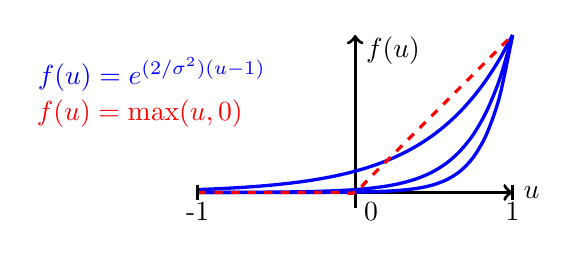
\begin{tikzpicture}[scale=2]
      \draw[->,very thick,black] (-1,0) -- (1,0) node[right] {$u$};
      \draw[->,very thick,black] (0,-0.1) -- (0,1) node[right,yshift=-2mm] {$f(u)$};
      \draw[scale=1,domain=-1:1,smooth,variable=\x,very thick,blue] plot ({\x},{exp(2*(\x-1))});
      \draw[scale=1,domain=-1:1,smooth,variable=\x,very thick,blue] plot ({\x},{exp(4*(\x-1))}) node[left,xshift=-3cm,yshift=-0.5cm] {$f(u)=e^{(2/\sigma^2)(u-1)}$};
      \draw[scale=1,domain=-1:1,smooth,variable=\x,very thick,blue] plot ({\x},{exp(6*(\x-1))});
      \draw[scale=1,domain=-1:1,smooth,variable=\x,very thick,dashed,red] plot ({\x},{max(\x,0)}) node[left,xshift=-3.29cm,yshift=-1cm] {$f(u)=\max(u,0)$};
      \draw (0,0) node[anchor=north,xshift=2mm] {0};
      \draw (1,0) node[anchor=north] {1};
      \draw (-1,0) node[anchor=north] {-1};
      \draw[very thick] (-1,0.05) -- (-1,-0.05);
      \draw[very thick] (1,0.05) -- (1,-0.05);
   \end{tikzpicture}
   \vspace*{-0.3cm}
   \caption{In dotted red, we plot the ``rectified linear unit'' function $u \mapsto \max(u,0)$. In blue, we plot non-linear functions of our network for typical values of~$\sigma$ that we use in our experiments.}\label{fig:relu}
\end{figure}

\vspace*{-0.3cm}
\subsection{Approximating the Multilayer Convolutional Kernel}

We have now all the tools in hand to build our convolutional kernel network.
We start by making assumptions on the input data, and then present the learning scheme and its approximation principles.

\vs
\paragraph{The zeroth layer.} We assume that the input data is a
finite-dimensional map $\xi_0: \Omega_0' \to \Real^{p_0}$, and that $\varphi_0:
\Omega_0 \to \HH_0$ ``extracts'' patches from~$\xi_0$. Formally, there
exists a patch shape~$\PP_0'$ such that $\Omega_0' = \Omega_0 + \PP_0'$, $\HH_0
= \Real^{p_0|\PP_0'|}$, and for all $\z_0$ in~$\Omega_0$, $\varphi_0(\z_0)$ is
a patch of $\xi_0$ centered at~$\z_0$. 
Then, property {\bfseries (B)} described at the beginning of
Section~\ref{sec:approx} is satisfied for $k\!=\!0$ by choosing
$\psi_0\!=\!\varphi_0$. The examples of input feature maps given earlier
satisfy this finite-dimensional assumption: for the gradient map, $\xi_0$ is
the gradient of the image along each direction, with $p_0=2$, $\PP_0'=\{ 0\}$
is
a $1 \!\times \!1$ patch, $\Omega_0\!=\!\Omega_0'$, and $\varphi_0\!=\!\xi_0$;
for the patch map, $\xi_0$ is the input image, say with $p_0\!=\!3$ for RGB data.


\vs
\paragraph{The convolutional kernel network.}
The zeroth layer being characterized, we present in Algorithms~\ref{alg:ckn}
and~\ref{alg:ckn2} the subsequent layers and how to learn their parameters 
in a feedforward manner. It is interesting to note that the input parameters of
the algorithm are exactly the same as a CNN---that is, number of layers and filters,
sizes of the patches and feature maps (obtained here via the subsampling factor).
Ultimately, CNNs and CKNs only differ in the cost function that is
optimized for learning the filters and in the choice of non-linearities.  As we
show next, there exists a link between the parameters of a CKN and those of
a convolutional multilayer kernel.

\begin{algorithm}
   \caption{Convolutional kernel network - learning the parameters of the $k$-th layer.}\label{alg:ckn}
   \begin{algorithmic}[1]
      \INPUT $\xi^1_{\kmone}, \xi^2_{\kmone},\ldots: \Omega'_{\kmone} \to \Real^{p_{\kmone}}$ (sequence of $(\kmone)$-th maps obtained from training images); $\PP_{\kmone}'$ (patch shape); $p_k$ (number of filters); $n$ (number of training pairs);
      \STATE extract at random $n$ pairs $(\x_i,\y_i)$ of patches with shape $\PP_{\kmone}'$ from the maps~$\xi_{\kmone}^1,\xi_{\kmone}^2,\ldots$;
      \STATE if not provided by the user, set $\sigma_k$ to the~$0.1$ quantile of the data~($\|\x_i-\y_i\|_2)_{i=1}^n$;
      \STATE {\bfseries unsupervised learning:} optimize~(\ref{eq:opt}) to obtain the filters~$\W_k$ in~$\Real^{|\PP_{\kmone}'|p_{\kmone} \times p_k}$ and $\etab_k$ in~$\Real^{p_k}$;
      \OUTPUT $\W_k$, $\etab_k$, and $\sigma_k$ (smoothing parameter);
   \end{algorithmic}
\end{algorithm}
\begin{algorithm}
   \caption{Convolutional kernel network - computing the $k$-th map form the~$(\kmone)$-th one.}\label{alg:ckn2}
   \begin{algorithmic}[1]
      \INPUT $\xi_{\kmone}: \Omega'_{\kmone} \!\to\! \Real^{p_{\kmone}}$ (input map); $\PP_{\kmone}'$ (patch shape); $\gamma_k \!\geq \!1$ (subsampling factor); $p_k$ (number of filters); $\sigma_k$ (smoothing parameter); $\W_k=[\w_{kl}]_{l=1}^{p_k}$ and~$\etab_k=[\eta_{kl}]_{l=1}^{p_k}$ (layer parameters);
      \STATE {\bfseries convolution and non-linearity:} define the activation map $\zeta_k: \Omega_{\kmone} \to \Real^{p_k}$ as
      \begin{equation}
         \vsb
         \zeta_k: \z \mapsto \|\psi_{\kmone}(\z)\|_2 \left[\sqrt{\eta_{kl}} e^{-\frac{1}{\sigma_k^2}\left\|\tildepsi_{\kmone}(\z)-\w_{kl}\right\|_2^2}\right]_{l=1}^{p_k}, \label{eq:zeta}
      \end{equation}
      where~$\psi_{\kmone}(\z)$ is a vector representing a patch from~$\xi_{\kmone}$ centered at~$\z$ with shape $\PP_{\kmone}'$, and the vector $\tildepsi_{\kmone}(\z)$ is an $\ell_2$-normalized version of~$\psi_{\kmone}(\z)$. This operation can be interpreted as a spatial convolution of the map~$\xi_{\kmone}$ with the filters~$\w_{kl}$ followed by pointwise non-linearities;
      \STATE set~$\beta_k$ to be~$\gamma_k$ times the spacing between two pixels in~$\Omega_{\kmone}$;
      \STATE {\bfseries feature pooling:}
      $\Omega'_k$ is obtained by subsampling~$\Omega_{\kmone}$ by a factor~$\gamma_k$ and we define a    
      new map $\xi_{k}: \Omega'_k \to \Real^{p_k}$ obtained from~$\zeta_k$ by linear pooling with Gaussian weights:
      \begin{equation}
         \vsb
         \xi_k: \z \mapsto \sqrt{{2}/\pi}\sum_{\u \in \Omega_{\kmone}}  e^{-\frac{1}{\beta_k^2}\left\|\u - \z\right\|_2^2} \zeta_k(\u). \label{eq:xi}
      \end{equation}
      \OUTPUT $\xi_{k} : \Omega'_k \to \Real^{p_k}$ (new map);
   \end{algorithmic}
\end{algorithm}

\paragraph{Approximation principles.}
\vspace*{-0.75cm}
We proceed recursively to show that the kernel approximation
property~{\bfseries (A)}
is satisfied; we assume that~{\bfseries (B)}
holds at layer~$\kmone$, and then, we show that {\bfseries (A)} and
{\bfseries (B)} also hold at layer~$k$.  This is sufficient for our 
purpose since we have previously assumed~{\bfseries (B)} for the zeroth layer.  
Given two images feature maps~$\varphi_{\kmone}$ and~$\varphi_{\kmone}'$, we 
start by approximating $K(\varphi_{\kmone},\varphi_{\kmone}')$ by replacing
$\varphi_{\kmone}(\z)$ and $\varphi_{\kmone}'(\z')$ by their finite-dimensional
approximations provided by~{\bfseries (B)}: 
\begin{equation}
   K(\varphi_{\kmone},\varphi_{\kmone}') \approx 
   \sum_{\z,\z' \in \Omega_{\kmone}} \normE{\psi_{\kmone}(\z)}  \normE{\psi_{\kmone}'(\z')} e^{-\frac{1}{2\beta_{k}^2}\normE{\z-\z'}^2} e^{-\frac{1}{2\sigma_k^2} \normE{\tildepsi_{\kmone}(\z)-\tildepsi_{\kmone}'(\z')}^2}.
\end{equation}
Then, we use the finite-dimensional approximation of the Gaussian kernel
involving~$\sigma_k$ and
\begin{equation}
         \vsb
   K(\varphi_{\kmone},\varphi_{\kmone}') \approx 
   \sum_{\z, \z' \in \Omega_{\kmone}} \zeta_k(\z)^\top \zeta_k'(\z') e^{-\frac{1}{2\beta_k^2}\normE{\z-\z'}^2},
\end{equation}
where~$\zeta_k$ is defined in~(\ref{eq:zeta}) and $\zeta_k'$ is defined
similarly by replacing~$\tildepsi$ by~$\tildepsi'$.  Finally, we approximate
the remaining Gaussian kernel by uniform sampling on $\Omega_{k}'$,
following Section~\ref{subsec:approx_gaussian}.
After exchanging sums and grouping appropriate terms together, we obtain the new approximation 
\begin{equation}
   K(\varphi_{\kmone},\varphi_{\kmone}') \approx \frac{2}{\pi} \sum_{\u \in \Omega_{k}'} \bigg( \sum_{\z \in \Omega_{\kmone}} e^{-\frac{1}{\beta_k^2}\normE{\z-\u}^2}\zeta_k(\z) \bigg)^\top \bigg( \sum_{\z' \in \Omega_{\kmone}}  e^{-\frac{1}{\beta_k^2}\normE{\z'-\u}^2} \zeta_k'(\z')  \bigg), \label{eq:approx}
\end{equation}
where the constant~$2/\pi$ comes from the multiplication of the constant
$2/(\pi\beta_k^2)$ from~(\ref{eq:rbf}) and the weight $\beta_k^2$ of uniform sampling
orresponding to the square of the distance between two pixels
of~$\Omega_k'$.\footnote{The choice of~$\beta_k$ in Algorithm~\ref{alg:ckn2} is
driven by signal processing principles. The feature pooling step can indeed be
interpreted as a downsampling operation that reduces the resolution of the map
from~$\Omega_{\kmone}$ to~$\Omega_k$ by using a Gaussian anti-aliasing filter,
whose role is to reduce frequencies
above the Nyquist limit.} As a result, the right-hand side is exactly $\langle
\xi_{k}, \xi_k' \rangle$, where~$\xi_k$ is defined in~(\ref{eq:xi}), giving us
property~{\bfseries (A)}. It remains to show that property~{\bfseries (B)} also
holds, specifically that the quantity~(\ref{eq:kernelpatch}) can be
approximated by the Euclidean inner-product~$\langle\psi_{k}(\z_k),
\psi'_k(\z_k')\rangle$ with the patches~$\psi_k(\z_k)$ and~$\psi'_k(\z_k')$ of shape~$\PP_k'$; we assume for that purpose that~$\PP_k'$ is a
subsampled version of the patch shape~$\PP_k$ by a factor~$\gamma_k$.

We remark that the kernel~(\ref{eq:kernelpatch}) is the same
as~(\ref{eq:kernel}) applied to layer~$\kmone$ by replacing~$\Omega_{\kmone}$
by~$\{\z_k\}+\PP_k$. By doing the same substitution in~(\ref{eq:approx}), we
immediately obtain an approximation of~(\ref{eq:kernelpatch}). Then, all
Gaussian terms are negligible for all~$\u$ and~$\z$ that are far from each
other---say when $\|\u-\z\|_2 \geq 2\beta_k$. Thus, we may replace the
sums~$\sum_{\u \in \Omega_k'}\sum_{\z,\z' \in \{\z_k\}+\PP_k}$ by~$\sum_{\u \in \{\z_k\}+\PP_k'}\sum_{\z,\z' \in \Omega_{\kmone}}$,
which has the same set of ``non-negligible'' terms. This yields exactly the
approximation $\langle\psi_{k}(\z_k), \psi'_k(\z_k')\rangle$.

\vs
\paragraph{Optimization.} 
Regarding problem~(\ref{eq:opt}), stochastic gradient descent
(SGD) may be used since a potentially infinite amount of training
data is available. However, we have preferred to use
L-BFGS-B~\cite{byrd1995} on $300\,000$ pairs of randomly selected training data
points, and initialize~$\W$ with the K-means algorithm. L-BFGS-B
is a parameter-free state-of-the-art batch method, which is not as
fast as SGD but much easier to use. We always run the L-BFGS-B algorithm for~$4\,000$ iterations, which seems to ensure
convergence to a stationary point. Our goal is to demonstrate the preliminary
performance of a new type of convolutional network, and we leave as future work
any speed improvement. 
\vsb
